\section{Compression Method Selection}
\label{sec:selection}

This section applies the relations of Section~\ref{sec:laws} to the choice of compression
configuration under a storage budget and tests that choice, fixed in advance, on references that
supplied it no outcome.

\subsection{Selection under Storage Constraints}
\label{sec:selection_rule}

Given a reference model, a capability and a budget, the decision is
\begin{equation}
(m^{*},\boldsymbol\theta_m^{*})=\arg\min_{m,\;\boldsymbol\theta_m\in\mathcal F_m(B)}\;
\widehat L_{m,c}(\mathbf x,\boldsymbol\theta_m),
\label{eq:selection}
\end{equation}
where $\mathcal F_m(B)$ holds the settings of method $m$ whose nominal storage, stored matrix
parameters rather than runtime memory or sparse indexing, falls within $B$. The final rule calls
the pruning and quantization relations of Section~\ref{sec:laws} on a seen state and their
source-free medians on a new one; for distillation, whose candidates are students of one fixed
recipe, it calls a regression on the student state for mathematics and pre-specified constants for code
and question answering (Appendix Table~\ref{tab:locked_rule}). The budget and pool forms of
Eq.~\ref{eq:kdforms} enter no selection; the selection results test the rule as specified, not those
forms. A workload needing several capabilities at once replaces $\widehat L_{m,c}$ by the largest loss increase
$\max_c[\widehat L_c(M)-L_c(M_0)]$. On the controlled panel,
the law-based choice selects the method of the measured best candidate in 96\%, 95\% and 73\% of 289
cells for mathematics, code and question answering. We then fixed a complete rule and its selection
maps in advance for four fresh Pythia states, where they come within 0.14 nats of the best candidate and below
quantization alone (Appendix Fig.~\ref{fig:rule_regret}). Its distillation candidates were historical, so a second confirmation trained new ones.

\subsection{Independent Evaluation}
\label{sec:selection_confirm}

\begin{figure}[t]
\centering

\includegraphics[width=5.5in]{figs/s3_validation_legend.pdf}\\[1pt]
\begin{subfigure}[t]{1.35in}\centering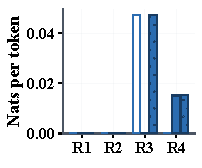
\includegraphics[width=\linewidth]{figs/s3_validation_a.pdf}\subcaption{Mathematics}\end{subfigure}\hfill
\begin{subfigure}[t]{1.35in}\centering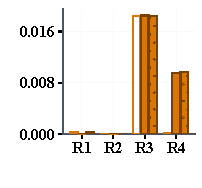
\includegraphics[width=\linewidth]{figs/s3_validation_b.pdf}\subcaption{Code}\end{subfigure}\hfill
\begin{subfigure}[t]{1.35in}\centering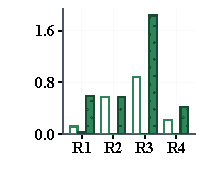
\includegraphics[width=\linewidth]{figs/s3_validation_c.pdf}\subcaption{Question answering}\end{subfigure}\hfill
\begin{subfigure}[t]{1.35in}\centering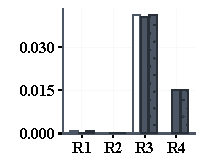
\includegraphics[width=\linewidth]{figs/s3_validation_d.pdf}\subcaption{Largest loss increase}\end{subfigure}
\caption{Independent validation of the final rule on four references that supplied it no outcome
(R1--R4: Pythia 410M and 1.4B at step 120000, Gemma 3 1B and 4B). Per objective: the
opportunity that choosing across methods opens over the best quantization candidate, and the regret
of the final rule and of a quantization-only policy, as means in nats per native token over the
sixteen budgets where both find a candidate. The earlier four-state confirmation is in Appendix
Figs.~\ref{fig:rule_maps} and \ref{fig:rule_regret}.}
\label{fig:rule_main}
\end{figure}


Each of the four references received twelve candidates at seventeen storage budgets: four pruning densities, six quantization settings, the
dense model and one student distilled in this round. Two are Pythia checkpoints with no earlier
recorded use; the two Gemma-3 models carry familiar weights and receive new candidates (Appendix
Table~\ref{tab:s3-identity}), with every predicted loss and both selection maps fixed before any
outcome was observed. The opportunity at a budget is the loss of the best feasible quantization
candidate minus that of the best feasible candidate of any method; a policy's regret is the loss of
its choice minus that same candidate. Question answering carries an opportunity of 0.12 to 0.89 nats (Fig.~\ref{fig:rule_main}a--d). Over all 68 question-answering cells, four references at seventeen budgets, the measured best
candidate is the new student in 59; of the other nine, three admit no feasible candidate, five
prefer pruning and one quantization. The two policies are compared on the 64 cells, sixteen budgets per
reference, at which both find a feasible candidate, and the rule selects the new student in 63 of
those. Its regret there is 0.000 nats on three references and 0.027 on the fourth, against 0.41 to
1.84 nats for a policy restricted to quantization, which also errs inside that family. For mathematics, code and the largest loss increase the opportunity is at most 0.047 nats;
quantization already supplies a near-best candidate, the rule matches it, and exceeds its regret in
three of the 256 paired cells by at most 0.0015 nats, all at the budget that admits the dense
model. All four references meet the criterion pre-specified for this round. A retrospective ablation on the same candidates (Appendix Table~\ref{tab:s3-ablation}) shows that
the rule's choices coincide with those of a development-fixed heuristic, the student first for
question answering and the largest feasible quantization otherwise, so they rest on a stable
difference between methods rather than on fine numerical margins; the development medians the rule
uses add to that on mathematics, 0.004 against 0.016 nats; and against a perfect quantization
selection the rule's choice is still better by 0.09 to 0.89 nats on question answering.

A retrospective control replaces the distilled student with the pristine one at the same nominal
storage: distillation raises the question-answering opportunity by 0.084 to 0.650 nats across the
four references and leaves mathematics and code unchanged or lower (Appendix
Table~\ref{tab:s3-retrospective-control}); these are changes in the candidate set's opportunity,
not in a student's own loss.
